\section{Алгоритъм}

\paragraph*{} Решението на задачата може да се раздели на две независими части - създаването на графа и обхождането му. Графа може да бъде създаден или като бъде прочетен от файл, който го описва, или като бъде генериран на случаен принцип.

\paragraph*{Прочитане на графа.} Това не е реализирано, макар че се изискваше от задачата. :(

\paragraph*{Генериране на графа.} Понеже се иска да генерираме случаен граф, т.е. без някаква определена структура, задачата може да се реши с просто прилагане на принципа паралелизъм по данни. Ако трябва да работим с n нишки, разделяме върховете на графа на n равни части и във всяка част генерираме $ 1 \over n $-та от ребрата. Всяка нишка може да работи в отделна част и не е необходима допълнителна синхронизация между тях.

\paragraph*{Обхождане на графа.} За случая с една нишка се използва стандартния последователен dfs алгоритъм. Това служи за база за сравнение. Основната трудност при многонишновия случай е, че трябва да запазим същата последователност на обхождане на върховете. За целта използваме една нишка, която прави обхождане в дълбочина, но без backtracking. Тоест започва от начален връх, преминава към първия му съсед, след това към първия съсед на съседа и т.н. докато не стигне до връх без повече необходени съседи. През всеки посетен връх, всички съседи освен първия се подават на допълнителни нишки, които правят същото обхождане. Това е визуализирано на фигура \ref{fig:algorithm}.

\paragraph*{} Идеята е докато една нишка обхожда графа, останалите да пробват останалите пътища. Ако в бъдеще първата нишка стигне до върхове обходени от някоя друга, то тези върхове трябва да бъдат обходени отново, защото е намерен ``по-къс'' път. Но ако това не се случи значи е намерен път, който е част от решението на задачата и в последователния алгоритъм би бил намерен при backtracking-а.

\paragraph*{} Този начин на обхождане налага за всеки връх да се пази не просто дали е обходен, ами от коя нишка е обходен. Освен това всяка проверка дали връх е вече посещаван трябва да се синхронизира с останалите нишки.

\begin{figure}[h]
  \centering
  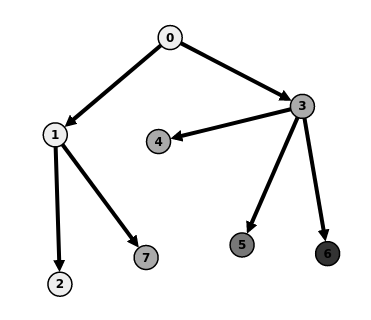
\includegraphics[width=0.5\textwidth]{resources/algorithm.png}
  \caption{\label{fig:algorithm} Разпределяне на търсенето по нишки. Върховете с един и същ цвят се обхождат от една и съща нишка.}
\end{figure}
